\documentclass[12pt]{article}
\usepackage{fancyhdr}
\usepackage{amsmath}
\usepackage{fancyvrb}
\usepackage{tikz}
\usepackage{caption}
\usepackage{amsthm}
\usepackage{booktabs}
\usepackage{wrapfig}
\usepackage{algorithm}% http://ctan.org/pkg/algorithms
\usepackage{algpseudocode}% http://ctan.org/pkg/algorithmicx
\usepackage{xcolor}
\usepackage[colorlinks = true,
            linkcolor = blue,
            urlcolor  = blue,
            citecolor = blue,
            anchorcolor = blue]{hyperref}
\usepackage{wrapfig}
\usepackage{setspace}
\usepackage{enumitem}
\usepackage[utf8]{inputenc}
\usepackage{tcolorbox}
\usepackage [english]{babel}
\usepackage [autostyle, english = american]{csquotes}
\MakeOuterQuote{"}
\usepackage{listings}
\usepackage{amssymb}
\usepackage[a4paper, left=1.5cm, right=1.5cm, top=2.5cm, bottom=1.5cm]{geometry}
\renewcommand{\thesection}{\Roman{section}} 
\renewcommand{\thesubsection}{\thesection.\Roman{subsection}}
\usepackage{titlesec}
\titleformat*{\section}{\fontsize{12}{5}\selectfont}
\titleformat*{\subsection}{\fontsize{12}{5}\selectfont}
\titlelabel{\thetitle.\enspace}
\usepackage{etoolbox}
\patchcmd{\thebibliography}{\section*}{\section}{}{}
\usepackage{fancyvrb}
\usepackage{gensymb}
\usepackage{pgfplots}
\pgfplotsset{compat=1.11}
\pagestyle{fancy}
\fancyhead{}
\fancyfoot{}
\fancyhead[L]{Evolutionary Time and Protein-Protein Interaction Networks}
\fancyhead[R]{STA 596}
\fancyfoot[C]{\thepage}
\usepackage{graphicx}
\usepackage{hyperref}
\usepackage{xcolor}

\usepackage{indentfirst}

\begin{document}
\title{\textbf{Evolutionary Time and Protein-Protein Interaction Networks}}
\author{Preliminary Analysis \\ \\ STA 596: Practical Data Science \\ Jesse Hautala \\ Shawn Houser \\ Angyalka Valcsics }

	\maketitle
\onehalfspacing

\noindent Contents
\begin{enumerate}[label = \Roman{*}.]
\item Introduction
\item Background
\item Methods
\item Preliminary Results
\item Conclusion
\item Appendix
\item References \newpage
\end{enumerate}

\section{Introduction}
Proteins control all biological systems in a cell and, through various interactions with each other, enable cells to complete tasks such as: enzyme activation, gene regulation, and intercellular communication. Protein interactions can be modeled by an undirected network of protein-protein interactions (a PPI network, or PPIN), with nodes representing proteins and edges representing interactions. The complete set of such interactions for a species is called the protein interactome. When interaction relationships between proteins break, possibly due to environmental factors or random mutations, such breakage can cause disease and death, of the cell and of the organism. We hypothesize that the evolutionary time of a species, which is defined by the total branch length from the root to the leaf representing that species in the tree of life, is directly related to network statistics which describe the topological stability of the species’ protein interactome.

\section{Background}
Advances in proteomics allow researchers to study the protein interactome, but limitations of experimental methods in practice prevent PPI networks from being comprehensive and free of noise. We regard extant PPIN data, including the data used in this project, as a noisy sample from the true protein interactome. For example, the yeast-two-hybrid method for mapping protein interactomes was first developed in 1989 by Fields and Song using \textit{Saccharomyces cerevisiae} as a biological model. The accuracy of this experimental method is estimated to be less than 10 percent. Consequently, the population being studied is the true protein interactome for each species and the variables of interest are the network statistics.

Understanding how protein interactomes evolve and developing methods for analyzing PPI networks is a central goal of evolutionary systems biology (Maddamsetti (2021)). In a paper by Rohan Maddamsetti they provided evidence that protein interactomes in E-Coli appear to show a generational increase in network resilience. Marinka Zitnik (Zitnik \textit{et al.} (2019)) defined network resilience as the measure of how quickly a network breaks down as edges between nodes are randomly removed. The current research identified a relationship between the resilience of an interactome and evolutionary time of the species.


\section{Methods}
\subsection{Acquisition of Data}
Our dataset comes from the Stanford Network Analysis Platform (or SNAP). This data was collected using the Search Tool for the Retrieval of Interacting Genes/Proteins (or STRING), from the European Molecular Biology Laboratory, EMBL and is organized in multiple text files, joined by species ID. It comprises taxonomy information, an edge set for each interactome, and a numerical variable for evolutionary time of the species. 

\begin{wrapfigure}{r}{0.5\textwidth}
  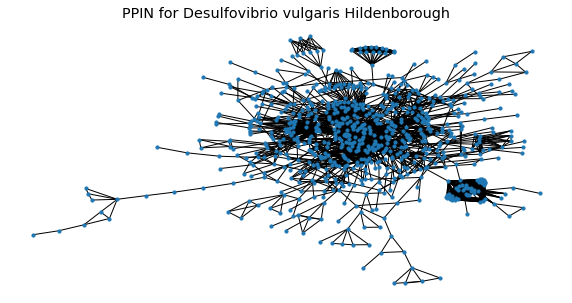
\includegraphics[width=0.95\linewidth]{PPIN_fig1}
\end{wrapfigure}

Shawn, creating the pickle is all you.

After transforming the data into a workable format, we selected an arbitrary subset of 75 species of Proteobacteria, a major phylum which includes a wide variety of pathogenic genera such as Salmonella. Our goal was to select a subset of networks which had a smaller size when compared to more complex species in the data since larger networks would increase computational time for our algorithms. 

Jesse, briefly we should both talk about how we got the two separate dfs with all of our network statistics. We can go into detail about the code in the appendix--you’ll see that I designated a section for it there. 


\subsection{Models}
Our research question aims to find network statistics, which measure topological stability of the species’ protein interactome, that are significant predictors of the evolutionary time of a species. That is, we suspect that there is a relationship between some of these network statistics and the response--evolutionary time. The nature of our data is that there are more features than data points. For this reason we need models that work well with such data--we need models which perform feature selection. 
Here I would like to explain what the ERGM is (using the pdf in the references below)   and how we used it, as well as explain how we concatenated the two dfs above together

\section{Preliminary Results}
LASSO info
Random forest info
\section{Conclusion}
Need to talk about how we plan to fine-tune the above models over the next two weeks here. I.e. Adding CV to lasso and tuning hyperparameters of random forest using RandomizedSearchCV.
\section{Appendix}
\subsection{Predictors Using NetworkX}

\begin{table}[H]
\centering
\caption{Predictors Using NetworkX Data Frame}
\begin{tabular}{lrrrrrr}
\toprule
Species\_ID &     882   &     883   &    36870 &    52598 &    56780  & $\cdots$\\
\midrule
Average Centrality       &     0.013 &     0.019 &    0.023 &    0.030 &    0.020 & $\cdots$\\
Average Closed Triangles &    51.938 &    47.910 &    9.525 &    1.058 &   62.323 & $\cdots$\\
Modularity               &     0.679 &     0.559 &    0.674 &    0.741 &    0.556 & $\cdots$\\
Clique Count             &  1060.000 &  3580.000 &  209.000 &  823.000 &  547.000 & $\cdots$\\
Clique-Size Max          &    26.000 &    19.000 &   10.000 &    6.000 &   27.000 & $\cdots$\\
Clique-Size Mode         &     2.000 &     5.000 &    2.000 &    2.000 &    2.000 & $\cdots$\\
Clique-Size Mean         &     4.726 &     5.004 &    2.923 &    2.335 &    4.075 & $\cdots$\\
LCSG Clique Count        &   916.000 &   371.000 &  180.000 &  249.000 &  451.000 & $\cdots$\\
LCSG Clique-Size Max     &    26.000 &    19.000 &   10.000 &    5.000 &   27.000 & $\cdots$\\
LCSG Clique-Size Mode    &     2.000 &     2.000 &    2.000 &    2.000 &    2.000 & $\cdots$\\
LCSG Clique-Size Mean    &     5.102 &     4.647 &    3.039 &    2.116 &    4.237 & $\cdots$\\
Node Count               &  1023.000 &   809.000 &  262.000 &  495.000 &  757.000 & $\cdots$\\
LCSG Node Count          &   736.000 &   502.000 &  217.000 &  139.000 &  536.000 & $\cdots$\\
LCSG Degree Max          &    60.000 &    58.000 &   27.000 &   11.000 &   66.000 & $\cdots$\\
LCSG Degree Mode         &     1.000 &     3.000 &    2.000 &    2.000 &    2.000 & $\cdots$\\
LCSG Degree Mean         &     9.465 &     9.661 &    5.060 &    4.144 &   10.590 & $\cdots$\\
\bottomrule
\end{tabular}
\end{table}
\subsection{K-Stars Algorithm}
Below it pseudocode for how we constructed the data frame of stars counts for each network.
\begin{algorithm}
\caption{Get Stars Algorithm}\label{alg:cap}
\begin{algorithmic}
\State $\text{giantC } \gets \text{ giant component for undirected network}$
\State $\text{A } \gets \text{ convert giantC to adjacency matrix}$
\State $\text{d } \gets \text{ sum row elements of A}$
\State $\text{values, counts } \gets \text{ find unique elements and counts for each}$
\State $\text{stars } \gets \text{ pandas DataFrame of counts with index names being values}$
\end{algorithmic}
\end{algorithm}
\begin{table}[H]
\centering
\caption{Count K-Stars Data Frame}
\begin{tabular}{lrrrrrr}
\toprule
Species\_ID &  882   &  883   &  36870 &  52598 &  56780 & $\cdots$\\
\midrule
num\_1stars &  109.0 &   39.0 &   22.0 &   17.0 &   26.0 & $\cdots$\\
num\_2stars &  105.0 &   57.0 &   54.0 &   30.0 &   70.0 & $\cdots$\\
num\_3stars &   65.0 &   63.0 &   31.0 &   20.0 &   53.0 & $\cdots$\\
$\vdots$ &   $\vdots$ &   $\vdots$ &   $\vdots$ &    $\vdots$ &   $\vdots$ & $\ddots$\\
\bottomrule
\end{tabular}
\end{table}
It is important to note that the maximum star count is unique to each network so when we concatenate these smaller data frames together to form the data frame which holds all network statistics it must be dynamic. Additionally, this means that once we train the model--if we choose to include all star variables--then we cannot test the model on a new set of networks. A quick fix for this may be to only include the first ten rows of this data frame. 
\begin{thebibliography}{1}
 \bibitem{1} Evolution of resilience in protein interactomes across the tree of life
Marinka Zitnik, Rok Sosič, Marcus W. Feldman, Jure Leskovec
bioRxiv 454033; doi: \url{https://doi.org/10.1101/454033}
\bibitem{2} Rohan Maddamsetti, Selection Maintains Protein Interactome Resilience in the Long-Term Evolution Experiment with Escherichia coli, Genome Biology and Evolution, Volume 13, Issue 6, June 2021, evab074, \url{https://doi.org/10.1093/gbe/evab074}
  \end{thebibliography}

%%%%%%%%%%%%%%%%%%%%%%%%%%%%%%%%%%%%%%%%%%%%%%%%%%%%%%%%%%%%%%%%%%%%%%%%%%%%%
\end{document}
